% ============================================================
% 分片：s03e  对应原文 PDF 第 47--50 页
% 负责章节：§3.2.3 Bulk local operators and Hochschild cohomology
%          （3.2.3 体局域算子与 Hochschild 上同调）
% 译者：translator-07   审校状态：初稿
% 图：figures/fig10.png（原文第 47 页，Figure 10）；figures/fig11.png、figures/fig12.png
%     （原文第 50 页，Figure 11、Figure 12）
% ============================================================
% [跨页接续: 原文第 46 页末句"…For example, we find that"续至第 47 页开头的公式；
%  本分片自该公式起接续，s03d 已译至"例如，我们发现"。]

% ==== 原文 PDF 第 47 页 ====

$f_1([\psi_1][\psi_2]) - f_1([\psi_1])f_1([\psi_2]) = \frac{1}{3}\phi^3 = \frac{1}{3}Q\partial_{\gamma_3}$，
这意味着可以取 $f_2([\psi_1],[\psi_2]) = \frac{1}{3}\partial_{\gamma_3}$。
对三元积 $\mu_3([\psi_1],[\psi_2],[\psi_3])$ 而言，其余相关的二元提升取为
$f_2([\psi_2],[\psi_3]) = \frac{1}{3}\partial_{\gamma_1}$，以及
% [存疑: 原文在此处把 $\partial_{\bar\gamma_n}$ 印作 $\partial_{\gamma_n}$（缺横线），
%  与 (3.28)、(3.29) 中的 $\partial_{\bar\gamma_n}$ 不一致；此处照抄原样，
%  疑为原稿记号疏漏，核对时以 $\partial_{\bar\gamma_n}$ 为准。]
\begin{equation}\tag{3.32}
\begin{aligned}
f_2([\psi_1],[\psi_2][\psi_3]) &= f_2([\psi_1],[\psi_2])\psi_3 - f_2([\psi_1],[\psi_3])\psi_2, \\
f_2([\psi_1][\psi_2],[\psi_3]) &= f_2([\psi_2],[\psi_3])\psi_1 - f_2([\psi_1],[\psi_3])\psi_2 .
\end{aligned}
\end{equation}
利用上述提升数据，式 (3.27) 给出
\begin{equation}\tag{3.33}
\mu_3([\psi_1],[\psi_2],[\psi_3]) = \frac{1}{3}
\end{equation}
这只需一段简短的运算即可得到。
% [Tutor Note: (3.33) 的结果与 (3.32) 中提升的选取无关：改变 $f_2\to f_2+Qg$ 会把右端改变一个
%  $Q$-恰当量，故上同调类不变。$\mu_3=\frac{1}{3}\neq 0$ 说明这个边界算子代数不是严格结合的：
%  $\psi_1(\psi_2\psi_3)$ 与 $(\psi_1\psi_2)\psi_3$ 之差并不为零，而是等于 $Q\mu_3(\psi_1,\psi_2,\psi_3)$
%  加上低阶项——高阶运算正是结合子的链级「修正项」。]

这个 $B$ 型扭变的 Landau--Ginzburg 模型与一个 $A$ 型扭变的 $\sigma$ 模型互为镜像，
后者的靶空间是三穿孔球面 [32, 81]。
三穿孔球面的（包裹的）Fukaya 范畴，即镜像 $A$ 型扭变理论中的边界条件范畴，
由 Figure 10 所示的三条拉格朗日（子流形）生成，其中每一条都镜像于上述生成元之一。
关于本例及其推广的同调镜像对称的补充分析见 [82--84]。
文献 [84] 给出了该范畴（的 $A_\infty$ 结构的一个极小模型）的具体描述，
并特别指出存在非零的三元运算 $\mu_3$（在此极小模型中）——该非零三元运算的贡献来自
Figure 10 中所画的全纯圆盘。物理上，$A$ 模型中的全纯圆盘对应于以相应拉格朗日子流形为边界的
世界面瞬子的贡献，因此比其 $B$ 模型对应物更难直接计算；更多细节见例如 [10]。
我们上面所作的三元积计算，正是这个非零三元运算的镜像。

\begin{figure}[tbp]
  \centering
  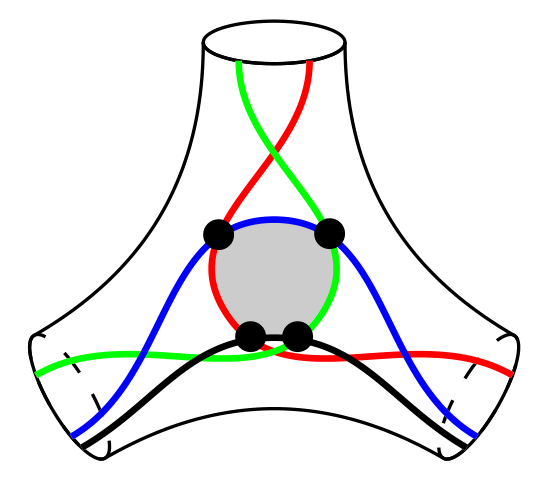
\includegraphics[width=0.92\linewidth]{figures/fig10.png}
  \caption{三穿孔球面及生成其包裹 Fukaya 范畴的三个拉格朗日子流形（红、蓝 $\sim$ 黑、绿）。
  阴影圆盘贡献一个 $A_\infty$ 三重积，它与非零三重积 $\mu_3(\psi_1,\psi_2,\psi_3)$ 互为镜像。
  （原文第 47 页，Figure 10）}
\end{figure}

\subsubsection{体局域算子与 Hochschild 上同调}

在转向全纯–拓扑混合情形之前，先回到这样一个问题：如何从拓扑边界条件范畴的信息
恢复体局域算子代数。正如 2.4.1 节所提到，局域算子代数预期可由膜范畴的 Hochschild 上同调恢复。
下面说明这一关系如何由拓扑下降产生：我们构造一个从体局域算子到
% ==== 原文 PDF 第 48 页 ====
Hochschild 上链的映射，它与扭变超荷 $Q$ 的作用以及 Hochschild 复形上的微分相容。
Hochschild 上同调自然具有 Gerstenhaber 代数结构 [85]，其中 Gerstenhaber 括号预期恢复
3.1.3 节所述的次级乘积；而（现已证明的）Deligne 猜想断言这可加强为完整的 $E_2$ 代数；
见例如 [73, Section 1.2] 及其中的文献。

我们首先回顾带有单个对象 $B$（或由单个对象 $B$ 生成）的范畴的 Hochschild 上同调这一概念，
并假设该对象的自同态 $\operatorname{Hom}_{\mathbf{Bdy}}(B,B)$ 由 DGA $(A,Q_\partial)$ 给出
（而不是、比如说，完整的 $A_\infty$ 代数）。于是我们关心 $A$ 的（系数在 $A$ 中的）
Hochschild 上同调，记作 $HH^\bullet(A) = HH^\bullet(A,A)$。
Hochschild $n$-上链是从 $A$ 的 $n$ 份到 $A$ 自身的多重线性映射：
\begin{equation}\tag{3.34}
HC^n(A) = \operatorname{Hom}_{\mathbb{C}}(A^{\otimes n}, A) .
\end{equation}
% [背景补充: Hochschild--Kostant--Rosenberg 定理断言，对光滑交换代数 $A$ 有
%  $HH^n(A)\cong\wedge^n\operatorname{Der}(A)$（多向量场）。这正是「体局域算子可由膜的范畴的
%  Hochschild 上同调恢复」的代数原型：$HH^\bullet$ 上的 Gerstenhaber 括号对应多向量场上的
%  Schouten 括号，故泊松结构（以及其量子化）可由 $HH^\bullet$ 读出。]
$HC^\bullet(A)$ 带有两个自然的分次：对 $n$-上链 $\phi\in HC^n(A)$，称其具有 Hochschild 次数 $n$；
若
\begin{equation}\tag{3.35}
F(\phi(O_1,\dots,O_n)) = |\phi| + F(O_1) + \dots F(O_n)
\end{equation}
则称其具有内次数 $|\phi|$。其中 $F$ 一如既往度量 $A$ 中的次数。
类似地，有两个自然的微分。第一个是由 $A$ 诱导的微分 $Q^*_\partial$，
它把内次数增加 $1$，但保持 Hochschild 次数不变：
\begin{equation}\tag{3.36}
\begin{aligned}
(Q^*_\partial\phi)(O_1,\dots,O_n) &= Q_\partial\phi(O_1,\dots,O_n) - (-1)^{|\phi|}\phi(Q_\partial Q_1,\dots,O_n) \\
&\quad + \dots + (-1)^{|\phi|+F(O_1)+\dots}\phi(O_1,\dots,Q_\partial O_n)) .
\end{aligned}
\end{equation}
% [原文疑误: (3.36) 第二项印作 $\phi(Q_\partial Q_1,\dots,O_n)$，按上下文应为
%  $\phi(Q_\partial O_1,\dots,O_n)$；且第二行末尾多出一个右括号
%  （印作"$\dots,Q_\partial O_n))$"）。此处照抄原样，建议把该项的 $Q_1$ 更正为 $O_1$，
%  并删去多余的右括号。]
% [Tutor Note: 推导补足：$Q^*_\partial$ 是 $A$ 的微分 $Q_\partial$ 在 $\operatorname{Hom}_{\mathbb{C}}
%  (A^{\otimes n},A)$ 上诱导的微分——它既作用于复合的像，也逐项作用于每个自变量（第二项起），
%  后者带 $(-1)^{|\phi|}$ 的 Koszul 符号，因为 $Q_\partial$ 是奇算子。]
第二个微分 $\delta$ 保持内次数不变，并把 Hochschild 次数增加 $1$：
\begin{equation}\tag{3.37}
\begin{aligned}
(\delta\phi)(O_1,\dots,O_{n+1}) &= (-1)^{|\phi|F(O_1)}O_1\phi(O_2,\dots,O_{n+1}) - \phi(O_1O_2,\dots,O_{n+1}) \\
&\quad + \dots + (-1)^n\phi(O_1,\dots,O_nO_{n+1}) + (-1)^{n+1}\phi(O_1,\dots,O_n)O_{n+1} .
\end{aligned}
\end{equation}
% [存疑: (3.37) 末项的符号印作 $(-1)^{n+1}$；不同文献对 Gerstenhaber 微分的末项符号约定不一
%  （亦有写作 $(-1)^{n}$ 者），故此处不断言为笔误。照抄原文，核对时以原文约定为准。]
此外，容易验证 $Q^*_\partial$ 与 $\delta$ 彼此反对易，故 DGA 的 Hochschild 复形自然是一个双复形。
Hochschild 上同调是该双复形关于全微分 $Q^*_\partial + \delta$ 的上同调；
Hochschild 上同调自然按 Hochschild 次数与内次数之和分次，我们称之为次数或总次数，记作 $F$：
$F(\phi) = |\phi| + n$。注意 0-上链与 $A$ 的元素等同，这与我们对 $F$ 的约定相容。
正是这个分次与我们的 TQFT 的 $\mathbb{Z}$ 分次相对应。
% [Tutor Note: 推导补足：$Q^*_\partial$ 与 $\delta$ 的反对易性等价于 $Q_\partial$ 是 $A$ 的乘积的导子
%  （即 (3.25)），可从这两条定义直接展开验证。双复形的总微分 $Q^*_\partial+\delta$ 满足
%  $(Q^*_\partial+\delta)^2 = 0$，其全上同调才是与体局域算子对应的 $HH^\bullet$；
%  只取 $\delta$（Hochschild 微分）得到的是 $HH^\bullet(A)$ 的同伦版，二者在 $Q$-上同调层面一致。]

给定次数的一般 Hochschild 上同调类将是内次数与 Hochschild 次数各不相同的元素之和，
在辨认体局域算子时应当预期出现这种情况。特别地，若体局域算子 $O$ 的次数为 $F(O)$，
则应把它实现为总次数为 $F(O)$ 的上链的形式和：
\begin{equation}\tag{3.38}
O \leftrightarrow hc_O = \sum_n hc^n_O, \qquad hc^n_O\in HC^n(A), \qquad |hc^n_O| = F(O) - n .
\end{equation}
我们把扭变超荷 $Q$ 在局域算子 $O$ 上的作用，与全微分 $Q^*_\partial+\delta$ 在
Hochschild 上链 $hc_O$ 上的作用等同起来：
\begin{equation}\tag{3.39}
hc^n_{QO} = Q^*_\partial hc^n_O + \delta hc^{n-1}_O ,
\end{equation}
% ==== 原文 PDF 第 49 页 ====
其中约定 $hc^{-1}_O = 0$。注意右端两项的 Hochschild 次数均为 $n$，内次数均为 $F(O)-n+1$，
故总次数为 $F(O)+1$，符合预期。
% [Tutor Note: 易错预警：检验 (3.39) 的次数时，$Q^*_\partial hc^n_O$ 的 Hochschild 次数仍为 $n$、
%  内次数比 $|hc^n_O| = F(O)-n$ 多 $1$；$\delta hc^{n-1}_O$ 的 Hochschild 次数为 $(n-1)+1 = n$、
%  内次数仍为 $F(O)-(n-1) = F(O)-n+1$。两项总次数因而都是 $F(O)+1 = F(QO)$，与 $Q$ 提高
%  总次数 $1$ 一致。这也是判断指标是否错位的最快检验。]

最后，我们构造实现从体局域算子到 Hochschild 上链复形的（上）链映射的上链 $hc^n_O$。
或许并不意外，$n=0$ 的映射对应于把体算子搬到边界 $B$，即它把 $1\in\mathbb{C}$ 送到 $O|_B\in A$：
\begin{equation}\tag{3.40}
hc^0_O(1) = O|_B .
\end{equation}
由此立即得到 $hc^0_{QO}(1) = (QO)|_B = Q_\partial(O|_B) = (Q^*_\partial hc^0_O)(1)$，符合预期。
我们把边界上的点 $t=0$ 看作半空间 $\mathbb{H}^2$ 上单点（开球）的构型空间
$C_{\mathbb{H}^2}(1)$ 中的 0-链 $\mathcal{B}_0(\epsilon)$。$n$ 更高时情形更有趣。
$n=1$ 时须用 $O$ 构造把边界局域算子送到边界局域算子的映射 $hc^1_O$。
对这样的边界局域算子 $O_1\in A$，考虑
\begin{equation}\tag{3.41}
hc^1_O(O_1) = \int_{\mathcal{B}_1(\epsilon)}(OO_1)^{(1)} = \int_{\mathcal{B}_1(\epsilon)}O^{(1)}O_1 ,
\end{equation}
其中 $\mathcal{B}_1(\epsilon)$ 是 Figure 11 中间一幅图所示的围道，视为半空间 $\mathbb{H}^2$ 上
一体点（开球）与一边界点（开半球）的构型空间 $C_{\mathbb{H}^2}(1;1)$ 中的 1-链。
直接应用下降方程与 Stokes 定理即得
\begin{equation}\tag{3.42}
\begin{aligned}
hc^1_{QO}(O_1) &= Q_\partial hc^1_O(O_1) - (-1)^{F(O)-1}hc^1_O(Q_\partial O_1)
+ (-1)^{F(O)F(O_1)}O_1O|_B - O|_BO_1 \\
&= (Q^*_\partial hc^1_O)(O_1) + (\delta hc^0_O)(O_1) ,
\end{aligned}
\end{equation}
符合预期。注意若 $O$ 是 $Q$-闭的、$O_1$ 是 $Q_\partial$-闭的，
则 $hc^1_O(O_1)$ 可看作 $O$ 与边界相碰撞的两种可能方式之间的同伦：
\begin{equation}\tag{3.43}
Q_\partial hc^1_O(O_1) = O|_BO_1 - (-1)^{F(O)F(O_1)}O_1O|_B .
\end{equation}
% [Tutor Note: 推导补足：(3.42) 的最后两项来自 Stokes 定理的边界项。把下降方程写成
%  $Q_\partial O^{(k)} = \mathrm{d}O^{(k-1)}$（总微分 $Q$ 在边界上的作用取 $Q_\partial$），
%  则 $\int_{\mathcal{B}_1(\epsilon)}Q_\partial(OO_1)^{(1)} = \pm\int_{\partial\mathcal{B}_1(\epsilon)}
%  (OO_1)^{(0)}$；圆盘的两端点分别给出 $O_1O|_B$ 与 $-O|_BO_1$，符号由把 $O|_B$ 移过 $O_1$ 的
%  Koszul 符号 $(-1)^{F(O)F(O_1)}$ 决定。]

类似地，$n=2$ 时可构造需要 $A$ 的两个元素的映射 $hc^2_O$：
\begin{equation}\tag{3.44}
hc^2_O(O_1,O_2) = \int_{\mathcal{B}_2(\epsilon)}(OO_1O_2)^{(2)} = \int_{\mathcal{B}_2(\epsilon)}O^{(2)}O_1O_2 ,
\end{equation}
其中 $\mathcal{B}_2(\epsilon)$ 是 Figure 11 右图所示的区域，视为一体点（开球）与
两个边界点（开半球）的构型空间 $C_{\mathbb{H}^2}(1;2)$ 中的 2-链。
再次直接应用下降方程与 Stokes 定理即得
\begin{equation}\tag{3.45}
hc^2_{QO}(O_1,O_2) = (Q^*_\partial hc^2_O)(O_1,O_2) + (\delta hc^1_O)(O_1,O_2) .
\end{equation}
于是若 $O$ 是 $Q$-闭的、$O_1,O_2$ 是 $Q_\partial$-闭的，则 $hc^2_O(O_1,O_2)$ 充当
把 $O|_B$ 移过 $O_1O_2$ 与先移过 $O_1$ 再移过 $O_2$ 这两种方式之间的同伦：
\begin{equation}\tag{3.46}
Q_\partial hc^2_O(O_1,O_2) = hc^1_O(O_1O_2)
- \left(hc^1_O(O_1)O_2 + (-1)^{(F(O)-1)F(O_1)}O_1hc^1_O(O_2)\right) .
\end{equation}
% [Tutor Note: 物理图像：(3.46) 度量的是体算子 $O$ 与边界算子乘积结合的「失效」程度——
%  把 $O|_B$ 一次性移过 $O_1O_2$，与分两步移过 $O_1$、$O_2$，两条路径相差的不是零而是 $Q_\partial$-恰当量，
%  该恰当性正是由 $hc^2_O$ 见证。这些同伦叠加起来给出体–边界映射在 $E_2$（而非 $E_1$）层面的结构，
%  即 Deligne 猜想所述的 Gerstenhaber/$E_2$ 代数结构。]

\begin{figure}[tbp]
  \centering
  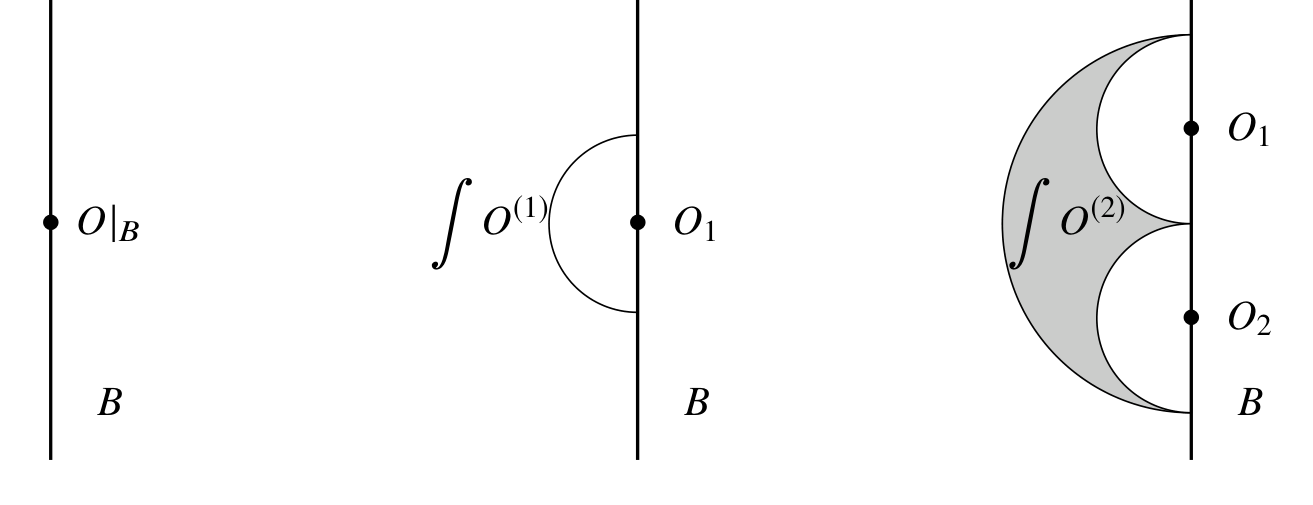
\includegraphics[width=0.92\linewidth]{figures/fig11.png}
  \caption{把体局域算子 $O$ 映为 Hochschild 上链 $hc_O$ 的前三个运算的图示。
  左：0-上链 $hc^0_O$ 来自边界值 $O|_B$，即沿 0-链 $\mathcal{B}_0(\epsilon)$ 的积分。
  中：1-上链 $hc^1_O$ 作用在边界局域算子 $O_1$ 上，来自把一阶后代 $O^{(1)}$ 沿
  1-链 $\mathcal{B}_1(\epsilon)$ 积分。右：2-上链 $hc^2_O$ 作用在边界算子 $O_1,O_2$ 上，
  来自把二阶后代 $O^{(2)}$ 沿 2-链 $\mathcal{B}_2(\epsilon)$ 积分。（原文第 50 页，Figure 11）}
\end{figure}

我们可以把这一过程系统化。正如 3.2.1 节所述的 $A_\infty$ 运算，我们构造一个多胞形，
其各个面编码上述同伦。在 Hochschild 次数
% ==== 原文 PDF 第 50 页 ====
$n$ 处，得到一个 $n$ 维多胞形，其 $n+1$ 个顶点对应于把 $O$ 与边界碰撞的
可能位置，例如 $O|_BO_1\dots O_n$ 或 $O_1O|_B\dots O_n$ 等等。1 维面（即棱）表示 $O|_B$
各种放置之间的同伦，并连接相差「把 $O|_B$ 移过单个算子（或单个算子乘积）」的顶点；
更一般地，$k$ 维面表示把 $O|_B$ 移过 $k$ 个边界算子（或 $k$ 个分离的算子乘积）的各种方式之间的
高阶同伦。上面已看到 $n=0$ 是点、$n=1$ 是区间、$n=2$ 是三角形；
一般地，相应的多胞形是 $n$-单形 $\Delta^n$。我们在 Figure 12 中展示 3-单形 $\Delta^3$
（即四面体）的情形，并在 Figure 13 中展示构型空间 $C_{\mathbb{H}^2}(1;3)$ 中相应的 3-闭链。
% [Tutor Note: 这里的多胞形与 $A_\infty$ 的 Stasheff 多胞形（结合多面体）形似而不同：结合多面体
%  的面编码 $n$ 元乘积的所有括号化方式，而此处编码的是体算子 $O|_B$ 在 $n$ 个边界算子之间的
%  所有插入位置（共 $n+1$ 个顶点）以及插入位置之间的移动同伦，故得到的是 $n$-单形 $\Delta^n$，
%  其真面个数 $2^{n+1}-2$ 与「插入位置子集」一一对应。]

\begin{figure}[tbp]
  \centering
  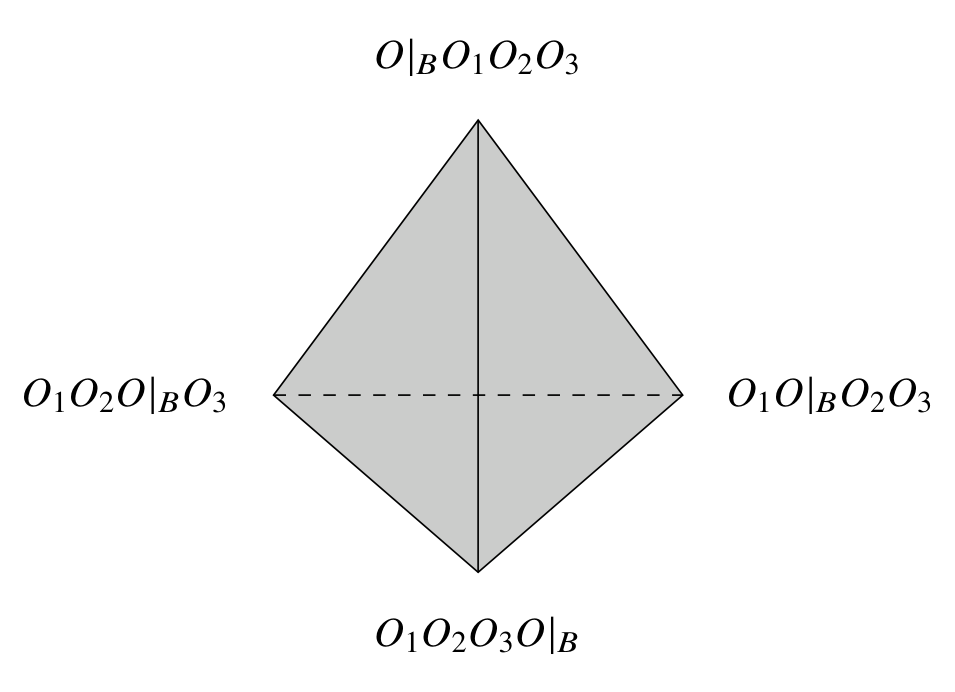
\includegraphics[width=0.92\linewidth]{figures/fig12.png}
  \caption{四面体 $\Delta^3$，其顶点用体局域算子 $O|_B$ 在边界局域算子 $O_1,O_2,O_3$ 之积中的
  位置来标记。四面体的棱对应于这些位置之间的同伦，例如虚线棱对应于 $O_1O|_BO_2O_3$ 与
  $O_1O_2O|_BO_3$ 之间由 $O_1hc^1_O(O_2)O_3$ 给出的同伦。四面体的面则对应于这些同伦之间的同伦，
  例如后面（rear face）对应于由 $hc^2_O(O_1,O_2)O_3$ 给出的、在
  $O|_B(O_1O_2)O_3\to(O_1O_2)O|_BO_3$ 与
  $O|_BO_1O_2O_3\to O_1O|_BO_2O_3\to O_1O_2O|_BO_3$ 之间的同伦。
  （原文第 50 页，Figure 12）}
\end{figure}

以此方式，我们可以通过对一个区域积分来构造具有 $n$ 个输入的多线性映射。
% [跨页接续: 原文第 50 页末句"In this fashion, we can construct a multilinear map with $n$ inputs
%  by integrating over a region"续至第 51 页"$\mathcal{B}_n(\epsilon)$ in the configuration space
%  $C_{\mathbb{H}^2}(1;n)$"，由 s03f 接续（该页 Figure 13 亦归 s03f）。]
